\documentclass[../../index.tex]{subfiles}

\begin{document}
\chapter{Introduction}
In particle physics we are concerned about small objects and their interactions.
Since the 1970 the dynamics of these tiny pieces are best described by the Standard Model (SM).

The SM contains two groups of fermionic, Spin 1/2 particles. The former group,
the Leptons consist of: the electron ($e$), the muon ($\mu$), the tau ($\tau$)
and their corresponding neutrinos $\nu_e$, $\nu_\mu$ and $\nu_\tau$. The latter
group, the Quarks contain: $u$, $d$ (up and down, the so called light quarks ),
$s$ (strange), $c$ (charm), $b$ (beauty or beauty) and $t$ (top or truth). The SM
furthermore differenciates between three fundamental forces (and its carriers):
the electromagnetic ($\gamma$ photon), weak ($Z$- or $W$-Boson) and strong ($g$
gluon) interactions. The before mentioned Leptons solely interact through the
electromagnetic and the weak force (also refered to as electroweak interaction),
whereas the quarks additionally interact through the strong force.

The strong force is denominated Quantumchromodynamics
(QCD). As the name suggest\footnote{Chromo is the greek word for color.} the
force is characterized by the color charge. Every quark has next to its type one
of the three colors blue, red or green. The color force is mediated through
eight gluons, which each being bi-colored\footnote{Each gluon carries a color
  and an anti-color.}, interact with quarks and each other. The strength of the
strong force is given by the coupling constant $\alpha_s$, which we will
determine within this work. The strong coupling constant $\alpha_s(E)$ is a function of energy $E$ and increases
with decreasing energies \footnote{In contrast to the electromagnetic force, where $\alpha(E)$
  decreases!}. This is exclusive for QCD and leads to \textit{asymptotic freedom} and
\textit{confinement}. The former phenomen describes the decreasing strong force
between quarks and gluons for high energies (short distances), which become asymptotically free at large
energies. The latter expresses the fact, that no isolated quark has been found
until today. Quarks appear confined as \textit{Hadrons}, the so called
\textit{Mesons}\footnote{Composite of a quark and an anti-quark.} and
\textit{Baryons}\footnote{Composite of three quarks or three anti-quarks.}.
As we measure \textit{Hadrons} in our experiments but calculate with quarks
within our theoretical QCD model we have to assume \textit{Quark-Hadron
  Duality}, which states that QCD, which is the theory of quarks and gluons, is still valid for Hadrons for energies
sufficently heigh. For lower energies there are measurable \textit{Duality Violations} (DV), which
will be commented within this work.

\textcolor{red}{taken from tau decay adapt!}
We are foremost interested into the hadronic decay channels, meaning
$\tau$-decays that have quarks in their final states. Unfortunately the quarks
have never been measured isolated, but appear always in combination of \textit{mesons}
and \textit{baryons}. Due to its mass of $m_\tau \approx
\SI{1.8}{\giga\electronvolt}$ the $\tau$-particle decays into light mesons
(pions-$\pi$, kaons-$K$, and eta-$\eta$, see \cref{table:lightMesons}), which
can be experimentally detected.
\begin{table}
  \centering
  \begin{tabular}{l c c c}
    \toprule
    Name & Symbol & Quark content & Rest mass ($\SI{}{\mega\electronvolt}$) \\
    \midrule
    Pion & $\pi^-$ & $\bar u d$ & \SI{139.57061 \pm 0.00024}{\mega\electronvolt}  \\
    Pion & $\pi^0$ & $(u \bar u - d \bar d)/\sqrt{2}$ & \SI{134.9770\pm0.0005}{\mega\electronvolt} \\
    Kaon & $K^-$ & $\bar u s$ & \SI{493.677\pm0.016}{\mega\electronvolt} \\
    Kaon & $K^0$ & $d \bar s$ & \SI{497.611\pm0.013}{\mega\electronvolt} \\
    Eta & $\eta$ & $(u \bar u + d \bar d - 2 s \bar s)/\sqrt{6}$ & \SI{547.862\pm0.017}{\mega\electronvolt} \\
  \end{tabular}
  \caption{List of mesons produced by a $\tau$-decay. Rare final states with
    branching Ratios smaller than 0.1 have been omitted. The list is taken from 
    \cite{Davier2006} with corresponding rest masses taken from \cite{PDG2018}.}
  \label{table:lightMesons}
\end{table}

In the following (\cref{sec:tauDecays}) we will describe the $\tau$-decays, which
play an essential role in our QCD analysis. Then in \cref{sec:quantumchromodynamics} we want to give more
details of QCD, especially about the coupling constant $\alpha_s(s)$ (which is not
constant at all) and the \textit{QCD sum rules}.


\section{Quantumchromodynamics}
\label{sec:quantumchromodynamics}
QCD gives a complete description of \textit{quarks} and \textit{gluons}. It is
born out of the very successful theory of \textit{quantum electrodynamics}
(QED), but has some major differences. QED has two well known constituent
fields the fermion and the photon. It is also a so called \textit{abelian}
theory, meaning that two consecutive rotations commute $AB = BA$. Due to the
abelian nature of the QED gauge group $U(1)$ only fermions carry gauge charge. Photons
do not carry charge. In contrast QCD takes quarks\footnote{Quarks are a subset
  to the fermions.} and gluons as fields. Additionally QCD is ruled by a \textit{non-abelian}
gauge symmetry of $SU(3)$. Thus the group operation of QCD in general do not
commute, which leads to gluons carrying charge! This charge is called
\textit{color-charge}. The theory requieres three colors and describes
interactions between a quark of a color with a quark of another color via
gluons. Contrary to QED the force carrier, the gluons, interact with themselve,
because they carry color charge.
\begin{table}
  \centering
  \begin{minipage}[c]{0.4\textwidth}
    \begin{tabular}{l l}
      \toprule
      Flavour & Mass\\
      \midrule
      $u$ & \SI{3.48(24)}{\mega\eV} \\
      $d$ & \SI{6.80(29)}{\mega\eV} \\
      $s$ & \SI{130.0(18)}{\mega\eV} \\
      $c$ & \SI{1.523(18)}{\giga\eV} \\
      $b$ & \SI{6.936(57)}{\giga\eV} \\
      $t$ & \SI{173.0(40)}{\giga\eV} \\
      \bottomrule 
    \end{tabular}
  \end{minipage}\hfill
  \begin{minipage}[c]{0.59\textwidth}
    \caption{List of Quarks and their masses. The masses of the up, down, strange,
      charm and bottom quark are the renormalization group invariant (RGI) quark
      masses and are quoted in the four-flavour theory ($N_f=2+1$) at
      the scale $\mu=\SI{2}{\giga\eV}$ in the $\overline{MS}$ scheme and are taken
      from the \textit{Flavour Lattice Averaging Group} \cite{FLAG2019}. The mass
      of the top quark is not disucess in \cite{FLAG2019} and has been taken from
      \cite{PDG2018} from direct observations of top events.}
  \end{minipage}
  \label{table:quarkList}
\end{table}

The theory of QCD can be summarized with its \textit{Lagrange density}\cite{Jamin2006}:
\begin{equation}
  \label{eq:qcdLagrangian}
  \mathcal{L}_{QCD}(x) = -\frac{1}{4}G_{\mu\nu}^a(x)G^{\mu\nu a}(x) + \sum_A \left[ \frac{i}{2} \bar{q}^A(x) \gamma^\mu \overleftrightarrow{D}_\mu q^A(x) - m_A\bar{q}^A(x) a^A(x) \right],
\end{equation}
where $q^A(x)$ represents the quark fields and $G_{\mu\nu}^a$ being the \textit{gluon field strength tensor} given by:
\begin{equation}
  \label{eq:gluonField}
  G_{\mu\nu}^a(x) \equiv \partial_\mu B_\nu^a(x) - \partial_\nu^a(x) + g f^{abc} B_\mu^b(x) B_\nu^c(x),
\end{equation}
where $B_\mu^a$ are the \textit{gluon fields}, given in the \textit{adjoint
  representation} of the SU(3) gauge group with $f^{abc}$ as \textit{structure
  constants}. Furthermore we have used $A, B, \dotsc = 0, \dotsc 5$ as flavour indices, $a,
b, \dotsc = 0, \dotsc, 8 $ as color indices and $\mu, \nu, \dotsc = 0, \dotsc 3$ as lorentz indices.




\subsection{Renormalisation Group}
The perurbations of the QCD Lagrangian \ref{eq:qcdLagrangian} lead to divergencies, which have to be
\textit{renormalized}. There are different aproaches to 'make' these
divergencies finite. The most popular one is \textbf{dimensional
  regularisation}.

In \textit{dimensional regularisation} we expand the four space-time dimensions
to arbitrary dimensions. Consequently the in QCD calculations appearing
$\textit{Feyman integrals}$ have to be continued to $D$-dimensions like
\begin{equation}
  \label{eq:dimRegFeynmanIntegral}
  \mu^{2\epsilon} \int \frac{\dif^D p}{(2\pi)^D}\frac{1}{[p^2-m^2+i0][(q-p)^2=m^2+i0]},
\end{equation}
where we introduced the scale parameter $\mu$ to account for the extra
dimensions and conserve the mass dimension of the non continued integral.

In addition \textit{physical quantities}\footnote{Observables that can be
  measured.} cannot depend on the renormalisation scale $\mu$. Thus the
derivative by $\mu$ of a general \textit{physical quantity} $R(q, a_s, m)$ that depends on the
external momentum q, the renormalised coupling $a_s\equiv\alpha_s/\pi$ and the
renormalized quark mass $m$ has to yield zero
\begin{equation}
  \label{eq:RGE}
  \mu \od{}{\mu}R(q, a_s, m) = \left[ \mu \pd{}{\mu} + \mu \od{a_s}{\mu} \pd{}{m} + \mu \od{m}{\mu} \pd{}{m} \right] R(q, a_s, m) = 0.
\end{equation}
\cref{eq:RGE} is referred to as \textbf{renormalization group equation} and
is the basis for defining the \textit{renormalisation group functions}:
\begin{align}
  \beta(a_s) &\equiv -\mu \od{a_s}{\mu} = \beta_1 a_s^2 + \beta_2 a_s^3 + \dots & \beta-\text{function}
  \label{eq:betaFunction} \\
  \gamma(a_s) &\equiv - \frac{\mu}{m} \od{m}{\mu} = \gamma_1 a_s + \gamma_2 a_s^2 + \dots & \text{anomalous mass dimension}.
  \label{eq:anomalousMassDimension}
\end{align}

\subsubsection{Running gauge coupling}
The $\beta$-function and the anomalous mass dimension are responsible for the
running of the strong coupling and the running of the quark mass respektively.
In this section we will shortly review the $\beta$-function and its implications
on the strong coupling, whereas in the following section we will discuss the
anomalous-mass dimension.

Regarding the $\beta$-function we notice, that $a_s(\mu)$ is not a constant, but
\textit{runs} by varying its scale $\mu$. Lets observe the running of the strong
coupling constant by integrating the $\beta$-function 
\begin{equation}
  \int_{a_s(\mu_1)}^{a_s(\mu_2)}\frac{\dif a_s}{\beta(a_s)} = - \int_{\mu_1}^{\mu_2} \frac{\dif \mu}{\mu} = \log \frac{\mu_1}{\mu_2}.
\end{equation}
To analytically evaluate the above integral we can approximate the $\beta$-function to first order, with the known
coefficient
\begin{equation}
  \beta_1 = \frac{1}{6}(11 N_c - 2 N_f),
\end{equation}
yielding
\begin{equation}
  a_s(\mu_2) = \frac{a_s(\mu_1)}{\left( 1 - a_s(\mu_1) \beta_1 \log\frac{\mu_1}{\mu_2} \right)}.
\end{equation}
As we have three colours $N_c=3$ and six flavours $N_f=6$ the first
$\beta$-function \ref{eq:betaFunction} is positive. Thus for $\mu_2>\mu_1$ $a_s(\mu_2)$ decreases
logarithmically and vanishes for $\mu_2 \to \infty$. This behaviour is known as
\textit{asymptotic freedom}.
The coefficients of the $\beta$-function are currently known up to the 5th
order and listed in the appendix \ref{sec:betaCoefficients}.

\subsubsection{Running quark mass}
Not only the coupling but also the masses carry an energy dependencies, which is
governed by the \textit{anomalou mass dimension} $\gamma(a_s)$.

The properties of the running quark mass can be derived similar to the gauge
coupling. Starting from integrating the \textit{anomalous mass dimension} \ref{eq:anomalousMassDimension}
\begin{equation}
  \log \frac{m(\mu_2)}{m(\mu_1)} = \int_{a_s(\mu_1)}^{a_s(\mu_2)} \dif a_s \frac{\gamma(a_s)}{\beta(a_s)}
\end{equation}
we can approximate the \textit{anomalous mass dimension} to first order and
solve the integral analytically \cite{Schwab2002}
\begin{equation}
  m(\mu_2) = m(\mu_1)\left( \frac{a(\mu_2)}{a(\mu_1)} \right)^{\frac{\gamma_1}{\beta_1}} \left( 1 + \mathcal{O}(\beta_2, \gamma_2) \right).
\end{equation}
As $\beta_1$ and $\gamma_1$ (see \ref{app:gammaCoefficients}) are positive the
quark mass decreases with increasing $\mu$.
The general relation between different scales is given by
\begin{equation}
  m(\mu_2) = m(\mu_1) \exp \left( \int_{a_s(\mu_1)}^{a_s(\mu_2)} \dif a_s \frac{\gamma(a_s)}{\beta(a_s)}  \right)
\end{equation}
and can be solved numerically to run the quark mass to the needed scale $\mu_2$.

QCD in general has a precision problem caused by uncertainties and largness of the strong
coupling constant $\alpha_s$. The fine-structure constant (the coupling constant
of QED) is known to eleven digits, whereas the strong coupling is only known to
about four. Furthermore for low energies the strong coupling constant is much
larger than the fine-structure constant. E.g. at the $Z$-mass, the standard mass
to compare the strong coupling, we have an $\alpha_s$ of $0.11$, whereas the
fine structure constant would be around $0.007$. Consequently to use PT we have to
calculate our results to much heigher orders, including tens of thousends of
Feynman diagrams, in QCD to achieve a precision equal to QED. For even lower
energies, around \SI{1}{\giga\eV}, the strong coupling reaches a critical value
of $\approx 0.5$ leading to a break down of PT.

In this work we try to achieve a higher precision in the value of $\alhpa_s$.
Our method to measure the strong coupling is called \textbf{QCD sum rules},
which by itself is based on a concept called the \texit{two-point function} for
which we will devote the following section.

\subsection{Two-Point function}
\label{sec:twoPointFunction}
The vacuum expectation value of the product of the conserved
noether current $J_\mu(x)$ at different space-times points $x$ and $y$ is known
as the \textbf{two-point function} (or simply \textbf{correlator})
\begin{equation}
  \label{eq:twoPointFunction}
  \Pi_{\mu\nu}(q^2) = \langle  0 | J_\mu(x) J_\nu(y) | 0 \rangle,
\end{equation}
where the noether current is given by
\begin{equation}
  J_\mu(x) = \anti{q}(x) \Gamma q(y)
\end{equation}
, where $\Gamma$ stands for one of the dirac matrices $\Gamma \in \{ 1,
i\gamma_5, \gamma_\mu, \gamma_\mu\gamma_5\}$, specifying the quantum number of
the current (S: \textit{scalar}, P: \textit{pseudo-Scalar}, V:
\textit{vectorial}, A: \textit{axial-vectorial}, respectively). 

The correlator tensor $\Pi_{\mu\nu}(q^2)$ can be lorentz decomposed to a scalar
function $\Pi(q^2)$. There are only two possible terms that can reproduce the
second order tensor $q_\mu q_\nu$ and $q^2 g_{\mu\nu}$. The sum of both
multiplied with two arbitrary functions $A(q^2)$ and $B(q^2)$ yields
\begin{equation}
  \Pi_{\mu\nu}(q^2) = q_\mu q_\nu A(q^2) + q^2 g_{\mu\nu} B(q^2).
\end{equation}
By making use of the \textbf{Ward-identity} \cite{Peskin1995}
\begin{equation}
  \label{eq:wardIdentity}
  q^\mu \Pi_{\mu\nu}(q^2) = q^\nu \Pi_{\mu\nu} = 0
\end{equation}
we can demonstrate, that the two arbitrary functions are related
\begin{equation}
  \begin{split}
    q^\mu q^\nu \Pi_{\mu\nu} &= q^4 A(q^2) + q^4 B(q^2) = 0 \\
    &\quad \implies A(q^2) = -B(q^2).
  \end{split}
\end{equation}
Thus redefining $A(q^2) \equiv \Pi(q^2)$ we expressed the correlator as a scalar function
\begin{equation}
  \Pi_{\mu\nu}(q^2) = (q_\mu q_\nu - q^2 g_{\mu\nu})\Pi(q^2).
\end{equation}

The scalar QCD two point function can then be related to the spectrum of
hadronic states. The correlator is then related to an integral over the
\textbf{spectral function} $\rho(s)$ via the \textit{Källén-Lehmann spectral
  representation} \cite{Kallen1952,Lehmann1954}, which is known since the early fities
\begin{equation}
  \label{eq:dispersionRelation}
  \Pi(q^2) = \int_0^\infty \dif s \frac{\rho(s)}{s - q^2 - i \epsilon}.
\end{equation}

Equation \ref{eq:dispersionRelation} is refered to as \textbf{dispersion relation} analogous to similar
relations which arise for example in electrodynamics and defines the
\textbf{spectral function} (a derivation can be found in \cite{Rafael1997})
\begin{equation}
  \label{eq:spectralFunction}
  \rho(s) = \frac{1}{\pi} \Ima \Pi(s).
\end{equation}

Until know we connected theoretical correlators with the measurable hadronic
spectrum. Nevertheless the analytic properties of the correlators have to be
discussed as the function has discontinuities.

The main contribution from the spectral function given in
\cref{eq:dispersionRelation} are the hadronic final states
\begin{equation}
  2 \pi \rho(m^2) = \sum_n \langle  0 | J_\mu(x) | n \rangle \langle n | J_\nu(y) \rangle (2 \pi^2)^4 \delta^{(4)}(p - p_n),
\end{equation}
which lead to a series of continuous poles on the positive real axis for the
two-point function, see Fig. \ref{fig:analyticStructureCorrelator}.
\begin{figure}[h]
  \centering
  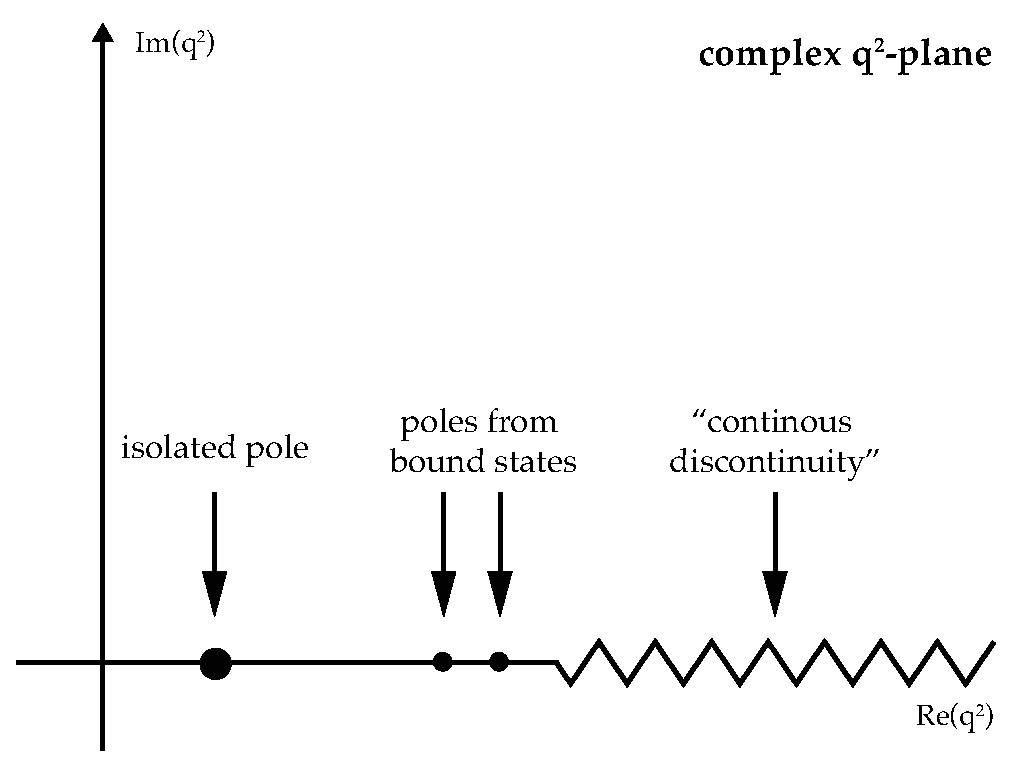
\includegraphics[width=0.8\textwidth]{./images/analyticStructureCorrelator.eps}
  \caption{Analytic structure in the complex $q^2$-plane of the Fourier
    transform of the two-point function. The hadronic final states are
    responsible for poles appearing on the real-axis. The one-particle states contribute as
    isolated pole and the multi-particle states contribute as bound-states poles
    or a continues ``discontinuity cut'' \cite{Peskin1995}.}
  \label{fig:analyticStructureCorrelator}
\end{figure}
These discontinuities can be tackled with \textit{Cauchy's theorem}, which we
will apply in \cref{secSumRules}.

Until now we exclusively dealt with the perturbative (PT) part of the theory,
but QCD is known to have not negligible non-perturbative (NPT) contributions.
Thus before continuing with the \textit{Sum Rules} we need a final ingredient
the operator product expansion, which implements NPT cotributions to our theory.


\subsection{Operator Product Expansion}
The \textbf{Operator Product Expansion} (OPE) was introduced by Wilson in 1969
\cite{Wilson1969}. The expansion states that non-local operators can be rewritten into a
sum of composite local operators and their corresponding coefficients:
\begin{equation}
  \label{eq:OPE}
  \lim_{x\to y} \mathcal{O}_1(x) \mathcal{O}_2(y) = \sum_n C_n(x-y)\mathcal{O}_n(x),
\end{equation}
where $C_n(x-y)$ are the so-called \textit{Wilson-coefficients}.

The OPE lets us separate \textit{short-distance} from \textit{long-distance}
effects. In perturbation theory (PT) we can only amount for
\textit{short-distances}, which are equal to hight energies, where the
strong-coupling $\alpha_s$ is small. Consequently the OPE decodes the
long-distance effects in the higher dimensionsional operators.

The form of the composite operators are dictated by Gauge- and Lorentz symmetry.
Thus we can only make use of operators of even dimension. The operators up to 
dimension six are given by \cite{Pascual1984}
\begin{equation}
  \begin{array}{ll}
    \text{Dimension 0:} & \mathbb{1} \\
    \text{Dimension 4:} & :m_i \anti{q} q: \\
                        & :G_a^{\mu\nu}(x) G_{\mu\nu}^a(x): \\
    \text{Dimension 6:} & :\anti{q} \Gamma q \anti{q} \Gamma q: \\
                        & :\anti{q} \Gamma \frac{\lambda^a}{2} q_\beta(x) \anti{q} \Gamma \frac{\lambda^a}{2} q: \\
                        & :m_i \anti{q} \frac{\lambda^a}{2} \sigma_{\mu\nu} q G^{\mu\nu}_a: \\
                        & :f_{abc} G_a^{\mu\nu} G_b^{\nu\delta} G_c^{\delta\mu}:,
  \end{array}
\end{equation}
where $\Gamma$ stands for one of the dirac matrices $\Gamma \in \{1, i \gamma_5,
\gamma^\mu, \gamma^\mu \gamma_5\}$, specifying the quantum number of the current
(S, P, A, respectively). As all the
operators appear normal ordered they vanish by definition in PT. Consequently
they appear as \textbf{Condensates} in Non-perturbative (NPT) QCD like
quark-condensate $\langle \anti{q} q \rangle$ or the gluon-condensate $\langle a
GG \rangle$ (both of dimension four). These non-vanishing condensats
characterize the QCD-vacuum.

As we work with dimensionless functions (e.g. $\Pi$) in Sum Rules, the r.h.s.
of \cref{eq:ope} has to be dimensionless. Consequently the
Wilson-coefficients have to cancel the dimension of the operator with their
inverse mass dimension. To account for the dimensions we can make the inverse
momenta explicit
\begin{equation}
  \Pi_{V/A}^{OPE}(s) = \sum_{D=0,2,4\dots} \frac{c^{(D)} \langle \mathcal{O}^{(D)}(x) \rangle}{-s^{D/2}},
\end{equation}
where we used $C^{(D)}=c/(-s)^{D/2}$ with $D$ being the dimension. Consequently
the OPE should converge with increasing dimension for suficienty large momenta $s$.

Let's show how the OPE contributions are calculated with a the
``standard example'' (following \cite{Pascual1986}), where we compute the
perturbative and quark-condensate Wilson-coefficients for the $\rho$-meson. 
For the $\rho$-meson, which is composed of u and d quarks, the current of \cref{eq:twoPointFunction} takes the
following form
\begin{equation}
  j^\mu(x) = \frac{1}{2}\left(:[\anti{u} \gamma^\mu u](x) - \anti{d} \gamma^\mu d](x)\right).
\end{equation}
\begin{figure}
  \centering
  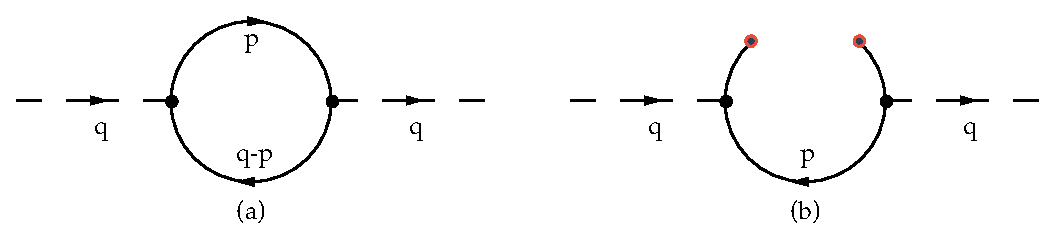
\includegraphics[width=\textwidth]{./images/condensateFeynmanDiagram.eps}
  \caption{Feynman diagrams of the perturbative (a) and the quark-condensate (b)
  contribution. The upper part of the right diagram is not wick-contracted and responsible for the condensate.}
  \label{fig:OPEFeynmanDiagram}
\end{figure}
In \cref{fig:OPEFeynmanDiagram} we draw the Feynman-diagram,
from which we can take the uncontracted mathematical expression for the scalar correlator
\begin{equation}
  \begin{split}
    \Pi(q^2) &= - \frac{i}{4 q^2 (D -1)} \int \dif^D x e^{iqx} \langle \Omega | T \{:\anti{u}(x) \gamma^\mu u(x) - \anti{d}(x) \gamma^{mu} d(x): \\
    &\quad\times :\anti{u}(0 \gamma_\mu u(0) - \anti{d}(0)\gamma_\mu d(0): \} \rangle.
  \end{split}
\end{equation}
Using Wick's theorem we can contract all of the fields and calculate the first
term of the OPE ($\mathbb{1}$), which represents the perturbative contribution
of the OPE ($\mathbb{1}$)
\begin{equation}
  \begin{split}
    \Pi(q^2) &= \frac{i}{4q^2(D-1)} (\gamma^\mu)_{ij} (\gamma_\mu)_{kl} \int \dif^D x e^{iqx} \\
    &\times\quad\left[
      \wick{ \c u_{j \alpha}(x) \anti{\c u}_{k \beta}(0)}
      \cdot \wick{\c u_{l \beta}(0) \anti{\c u}_{i \alpha}(x)} + (u \to d)
    \right] \\
    &= \frac{3}{8\pi^2} \left[ \frac{5}{3} - \log\left( -\frac{q^2}{\nu^2} \right) \right].
  \end{split}
\end{equation}

To calculate the higher dimensional contributions of the OPE we use the same
techniques as before, but leave some of the fields uncontracted. For the
quark-condensate, which we want to derive for tree-level, we leave two fields uncontracted
\begin{equation}
  \begin{split}
    \Pi(q^2) &= \frac{i}{4q^2(D-1)} (\gamma^\mu)_{ij} (\gamma_\mu)_{kl} \int \dif^D x e^{iqx} \left[ \phantom{\wick{ \c u_{j \alpha}(x) \anti{\c u}_{k \beta}(0)}} \right.\\
      &\quad+\,\wick{ \c u_{j \alpha}(x) \anti{\c u}_{k \beta}(0)} \cdot \langle \Omega \vert : \anti{u}_{i \alpha}(x) u_{l \beta} (0) :\vert \Omega \rangle \\
      &\quad\,\left.+\wick{\c u_{l \beta}(0) \anti{\c u}_{i \alpha}(x)} \cdot \langle \Omega \vert: \anti{u}_{k \beta}(0) u_{j \alpha}(x) : \vert \Omega \rangle + (u \to d)
    \right].
  \end{split}
\end{equation}
The non contracted fields can then be expanded in x
\begin{equation}
  \begin{split}
    \langle \Omega \vert: \anti{q}(x) q(0):\vert \Omega \rangle &= \langle\Omega\vert: \anti{q}(0) q(0): \vert\Omega\rangle\\
    &\quad+ \langle\Omega\vert:\left[ \partial_\mu \anti{q}(0) \right] q(0):\vert\Omega\rangle x^\mu + \dots
  \end{split}
\end{equation}
and redefined to a more elegant notation
\begin{equation}
  \langle \anti{q}q \rangle \equiv \langle\Omega\vert: \anti{q}(0) q(0):\vert\Omega\rangle.
\end{equation}
The finally result can be taken from \cite{Pascual1984} and yields
\begin{equation}
  \Pi_{(\rho)}(q^2) = \frac{1}{2} \frac{1}{\left(-q^2\right)^2} \left[ m_u\langle \anti{u} u + m_d \langle \anti{d} \rangle\right].
\end{equation}

The usage of the OPE and its validity is far from obvious. We are deriving the
OPE from matching the Wilson-coefficients to Feynman-graph analyses. These
Feynman-graphs are calculated perturbatively but the coefficients with dimension
$D>0$ correspond to NPT condensates!

Having gathered all of the necessary concepts we can close the gap between the
theory and experiment in the last section of the introduction: QCD Sum Rules.

\subsection{Sum Rules}
\label{sec:sumRules}
To relate the measurable hadronic final states of a QCD process (e.g.
$\tau$-decays into Hadrons) to a theoretical calculable \textbf{QCD sum rules}
have been empliyed by Shifman in the late sevent \cite{Shifman1978}.

The sum rules are a combination of the two-point function and its analyticity,
the OPE, a dispersion relation, the optical theorem and quark hadron duality.  

The previously introduced two-point function \cref{eq:twoPointFunction} is
generally descriped by the OPE to account for NPT effects.
\begin{equation}
  \Pi(q^2) = \Pi^{OPE}(q^2).
\end{equation}
Furthermore it is related to the theoretical spectral function $\rho(s)$ via a
dispersion relation \cref(eq:dispersionRelation). Using QCD we are computing
interactions based on quarks and gluons, but due to
confinement, we are only able to observe Hadrons. Consequently to connect the
theory to the experiment we have to assume \textbf{quark-hadron
  duality}\footnote{Or simply duality.}, which
implies that physical quantities can be described equally good in the hadronic or in
the quark-gluon picture. Thus we can rewrite the dispersion relation
\cref{eq:dispersionRelation} as
\begin{equation}
  \Pi^{OPE}_{th}(q^2) = \int_0^\infty \frac{\rho_{exp}(q^2)}{(s-q^2-i\epsilon)},
\end{equation}
where we connected the theoretical correlator $\Pi_{th}$ with the experimental
measurable spectral function $\rho_{exp}$.

We have seen that the theoretical description of the correlator $\Pi_{th}$
contains poles on the real axis, but the experimental data $\rho_{exp}$ is solely
accesible on the positive real axis. Thus we have to make
use of Cauchy's theorem to access the theoretical values of the two-point function close to the
postive real axis (see \cref{fig:correlatorComplexContour}) given by
\begin{equation}
  \label{eq:cauchysTheorem}
  \int_{\mathcal{C}} f(z) \dif z = 0,
\end{equation}
where $f(z)$ is an analytic function on a closed contour $\mathcal{C}$.
\begin{figure}[h]
  \centering
  \label{fig:correlatorComplexContour}
  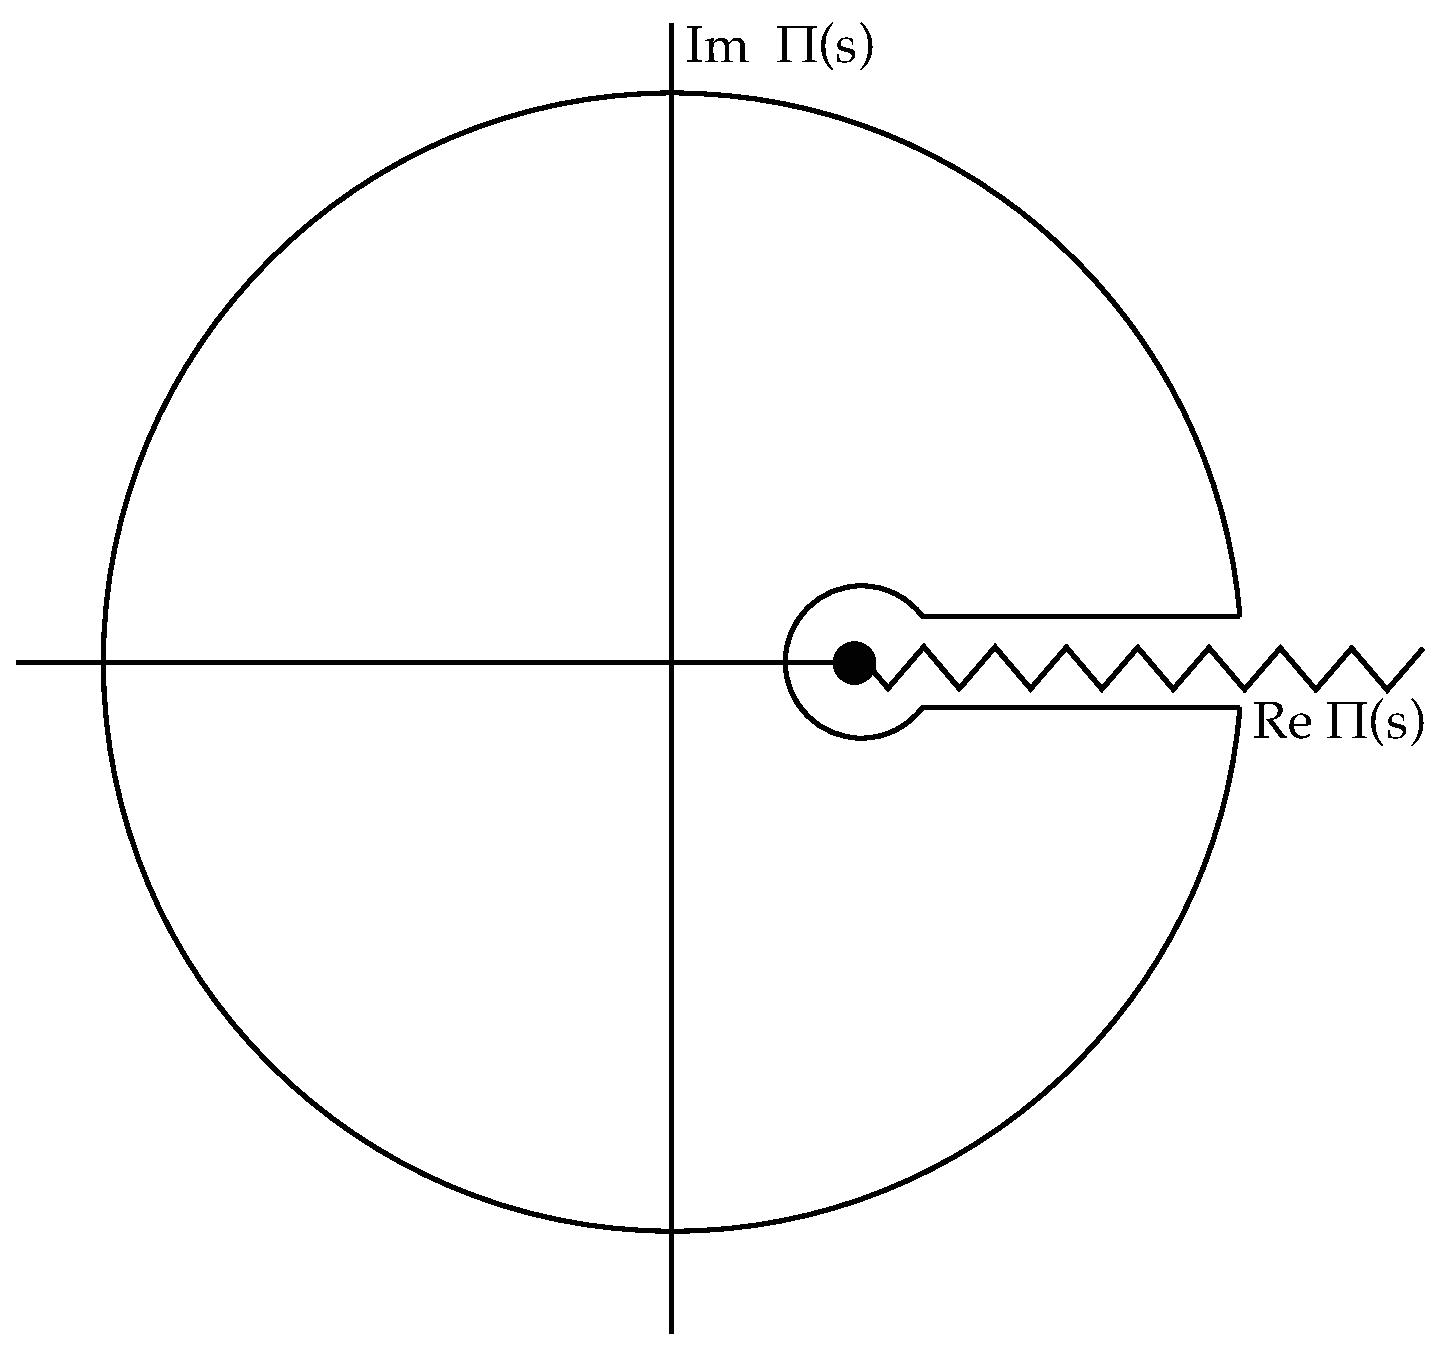
\includegraphics[width=0.6\textwidth]{./images/correlatorComplexContour.eps}
  \caption{Analytical structure of $\Pi(s)$ with the used contour $\mathcal{C}$
    for the final QCD Sum Rule expression \cref{eq:qcdSumRules}.}
\end{figure}

The final ingredient of the QCD sum rules is the \textit{optical theorem},
relating experimental data with the imaginary part of the correlator (the
spectral function $\rho(s)$). 

In total, with the help Cauchy's theorem, the QCD sum rules can be sumed up in
the following expression
\begin{equation}
  \label{eq:qcdSumRules}
  \frac{1}{\pi}\int_0^\infty \frac{\rho_{exp}(t)}{t - s}\dif t = \frac{1}{\pi} \oint_{\mathcal{C}} \frac{\Ima \Pi_{OPE}(t)}{t -s}\dif t,
\end{equation}
where the l.h.s. is given by the experiment and the r.h.s. can be theoretically
evaluated with by applying the OPE of the correlator $\Pi_{OPE}(s)$.
\end{document}